% !TEX root = ../OT4ML.tex

%%%%%%%%%%%%%%%%%%%%%%%%%%%%%%%%%%%%%%%%%%%%%%%%%%%%%%%%%%%%%%%%%%%%%%%%%%%
%%%%%%%%%%%%%%%%%%%%%%%%%%%%%%%%%%%%%%%%%%%%%%%%%%%%%%%%%%%%%%%%%%%%%%%%%%%
%%%%%%%%%%%%%%%%%%%%%%%%%%%%%%%%%%%%%%%%%%%%%%%%%%%%%%%%%%%%%%%%%%%%%%%%%%%
\chapter{Dual Problem}
\index{dual!problem}% strictindex
\label{sec-dual}

Duality turns the transport problem into a search for potentials rather than couplings. This chapter explains why potentials certify optimality, how $c$-transforms regularize them, and why the quadratic case reveals convex analysis behind Brenier maps. Linear-programming duality gives the discrete picture~\cite{bertsimas1997introduction}, while the continuous form is one of the central theorems of OT~\cite{Villani03,SantambrogioBook}.
\index{Brenier!map}% strictindex
\index{c-transform}% strictindex

%%%%%%%%%%%%%%%%%%%%%%%%%%%%%%%%%%%%%%%%%%%%%%%%%%%%%%%%%%%%%%%%%%%%%%%%%%%
\section{Discrete dual}


The discrete dual gives finite-dimensional certificates of optimality. Its complementary slackness conditions identify where an optimal coupling can put mass.
\index{optimal coupling}% strictindex
\index{optimality!complementary slackness}% strictindex

The Kantorovich problem~\eqref{eq-kanto-discr} is a linear program so that one can equivalently compute its value by solving a dual linear program.
\index{Kantorovich!problem}% strictindex

% a constrained convex minimization problem, and as such, it can be naturally paired with a so-called dual problem, which is a constrained concave maximization problem. The following fundamental proposition, which is a special case of Fenchel-Rockafellar duality theory, explains the relationship between the primal and dual problems.

\begin{defn}[Admissible potentials]\label{def-admissible-potentials}
\index{admissible!potential}% strictindex
\index{dual!potential}% strictindex
	For a discrete problem with marginal sizes $n,m$ and cost matrix $\C\in\RR^{n\times m}$, a pair $(\fD,\gD)\in\RR^n\times\RR^m$ is admissible if it lies below the cost:
	\eql{\label{eq-feasible-potential}
		\PotentialsD(\a,\b) \eqdef \enscond{
			(\fD,\gD) \in \RR^n \times \RR^m
		}{ \foralls (i,j) \in \range{n} \times \range{m}, \fD_i+\gD_j \leq \C_{i,j} }.
	}
	Equivalently, $\fD\oplus\gD\leq\C$ entrywise. The notation suppresses the dependence on $\C$, which is fixed in the surrounding problem.
\end{defn}
The two vectors play the role of source and target prices; admissibility means that no transported pair is priced above its travel cost.

\begin{prop}[Discrete Kantorovich duality]\label{prop-duality-discr}
\index{Kantorovich!duality}% strictindex
One has
\eql{\label{eq-dual}
	\MKD_\C(\a,\b) =
	\umax{(\fD,\gD) \in \PotentialsD(\a,\b)} \dotp{\fD}{\a} + \dotp{\gD}{\b}
}
\end{prop}

\begin{proof}
%
For the sake of completeness, let us derive this dual problem using Lagrangian duality. The Lagrangian associated to~\eqref{eq-kanto-discr} reads
\index{dual!problem}% strictindex
\eql{\label{eq-mk-lagr}
	\umin{\P \geq 0} \umax{ (\fD,\gD) \in \RR^n \times \RR^m }
		\dotp{\C}{\P} + \dotp{\a - \P\ones_m}{\fD} + \dotp{\b - \P^\top \ones_n}{\gD}.
}
For a linear program, if the primal constraint set is non-empty, one can always exchange the min and the max and get the same value. We thus consider
\eq{
	\umax{ (\fD,\gD) \in \RR^n \times \RR^m }
	\dotp{\a}{\fD} + \dotp{\b}{\gD}
	+ \umin{\P \geq 0}
		\dotp{\C - \fD\ones_m^\top - \ones_n \gD^\top}{\P}.
}
We conclude by remarking that
\eq{
	\umin{\P \geq 0} \dotp{\Q}{\P} =
	\choice{
		0 \qifq \Q \geq 0\\
		-\infty \quad \text{otherwise}
	}
}
so that the constraint reads $\C - \fD\ones_m^\top - \ones_n \gD^\top = \C-\fD\oplus \gD \geq 0$.
\end{proof}

The primal-dual optimality relation for the Lagrangian~\eqref{eq-mk-lagr} allows locating the support of the optimal transport plan
\index{support}% strictindex
\index{plan!transport}% strictindex
\eql{\label{eq-mk-pd-rel}
	\Supp(\P) \subset \enscond{(i,j) \in \range{n} \times \range{m}}{ \fD_i+\gD_j=\C_{i,j} }.
}

Figure~\ref{fig:dual-kantorovich-discrete-potentials} shows these finite-dimensional certificates on a one-dimensional quadratic problem.  The potentials are not transport maps themselves; rather, their contact set with the cost matrix is where an optimal coupling is allowed to put mass.
\index{cost matrix}% strictindex
\index{optimal coupling}% strictindex
\index{transport map}% strictindex

\begin{figure}[ht]
\centering
\begin{tabular}{@{}ccc@{}}

\includegraphics[width=.30\linewidth]{figures/dual-kantorovich-discrete-potentials/target-balanced.pdf} &

\includegraphics[width=.30\linewidth]{figures/dual-kantorovich-discrete-potentials/target-shifted.pdf} &

\includegraphics[width=.30\linewidth]{figures/dual-kantorovich-discrete-potentials/target-three-mode.pdf} \\[-.1em]
\small balanced target &
\small strongly shifted target &
\small three-mode target
\end{tabular}
\caption{Discrete Kantorovich dual potentials for the quadratic cost $C_{i,j}=|x_i-y_j|^2$.  In each panel the upper strip shows the fixed source histogram in red and the target histogram in blue: a balanced bimodal target, a more strongly shifted target, and a three-component mixture.  The lower strip shows an optimal pair of dual vectors $(\fD,\gD)$, with gauge chosen so that $\dotp{\fD}{\a}=0$.  Complementary slackness states that mass can be transported only through entries where $\fD_i+\gD_j=C_{i,j}$.}
\index{optimality!complementary slackness}% strictindex
\index{dual!potential}% strictindex
\index{cost!quadratic}% strictindex
\label{fig:dual-kantorovich-discrete-potentials}
\end{figure}

The formulation~\eqref{eq-dual} shows that $(\a,\b) \mapsto \MKD_\C(\a,\b)$ is a convex function (as a supremum of linear functions). From the primal problem~\eqref{eq-kanto-discr}, one also sees that $\C \mapsto \MKD_\C(\a,\b)$ is concave.
\index{convex!function}% strictindex

%%%%%%%%%%%%%%%%%%%%%%%%%%%%%%%%%%%%%%%%%%%%%%%%%%%%%%%%%%%%%%%%%%%%%%%%%%%
\section{Auction Algorithm and Dual Prices}
\index{auction algorithm}% strictindex
\index{dual!price}% strictindex
\label{sec-auction-dual-ascent}

The assignment algorithms mentioned in Chapter~\ref{sec-matching} become more transparent once one has dual variables. The auction algorithm is a dual price method: it updates target prices and maintains an approximate complementary-slackness certificate. The small tolerance $\epsilon$ removes ties, stabilizes the price updates and gives a quantitative optimality certificate~\cite{bertsekas1981new,bertsekas1992auction,merigot2020optimaltransportalgorithms}.
\index{optimality!certificate}% strictindex
\index{optimality!complementary slackness}% strictindex
\index{auction algorithm}% strictindex

Consider the square assignment problem with costs $C_{i,j}$ and rewrite it as the profit maximization problem with $a_{i,j}=-C_{i,j}$. The auction algorithm keeps prices $p_j$ on the target points and a partial assignment. For an unassigned source $i$, define the best and second-best reduced profits
\index{assignment problem}% strictindex
\[
	v_i=\max_j (a_{i,j}-p_j),\qquad
	j_i\in\operatorname*{argmax}_j(a_{i,j}-p_j),\qquad
	w_i=\max_{j\neq j_i}(a_{i,j}-p_j).
\]
Source $i$ bids for $j_i$ and increases its price by the gap to the second-best target, plus a margin:
\[
	p_{j_i}\leftarrow p_{j_i}+v_i-w_i+\epsilon.
\]
The target $j_i$ is then assigned to $i$, and its previous owner, if any, becomes unassigned. The iteration stops when all sources are assigned. Algorithm~\ref{alg:auction-bidding} records the bidding loop. Figure~\ref{fig:dual-auction-progression} displays actual auction iterates using the same assignment-state convention as Figure~\ref{fig:matching-hungarian-progression}: flat rows denote unassigned bidders, and one-hot rows denote currently owned targets.
\index{Hungarian primal-dual method}% strictindex

\begin{alg}[Auction bidding with target prices]\label{alg:auction-bidding}
\textbf{Input:} Profit matrix $A=(a_{ij})$, bid increment $\epsilon>0$.

\textbf{Output:} Assignment map $\sigma$.

\textbf{Initialize:} Set prices $p_j=0$.

\textbf{Mark} all sources and targets as unassigned.

\textbf{While} some source $i$ is unassigned \textbf{do}:
\begin{algblock}
\[
	v_i=\max_j(a_{ij}-p_j),
	\qquad
	j_i\in\argmax_j(a_{ij}-p_j),
	\qquad
	w_i=\max_{j\neq j_i}(a_{ij}-p_j).
\]
\textbf{Update price:}
\[
	p_{j_i}\leftarrow p_{j_i}+v_i-w_i+\epsilon.
\]
\textbf{If} target $j_i$ has owner $i'$ \textbf{then}:
\begin{algblock}

\textbf{Mark} $i'$ as unassigned.

\end{algblock}
\textbf{Assign} target $j_i$ to source $i$.

\end{algblock}
\textbf{Return} $\sigma$ induced by the target owners.
\end{alg}

\begin{figure}[ht]
\centering
\setlength{\tabcolsep}{2pt}
\begin{tabular}{ccccc}

\includegraphics[width=.18\linewidth]{figures/dual-auction-progression/stage-0.pdf} &

\includegraphics[width=.18\linewidth]{figures/dual-auction-progression/stage-1.pdf} &

\includegraphics[width=.18\linewidth]{figures/dual-auction-progression/stage-2.pdf} &

\includegraphics[width=.18\linewidth]{figures/dual-auction-progression/stage-3.pdf} &

\includegraphics[width=.18\linewidth]{figures/dual-auction-progression/stage-4.pdf} \\[-.1em]
\small initial &
\small 2 bids &
\small 5 bids &
\small 7 bids &
\small final
\end{tabular}
\caption{Matrix view of actual auction iterates on the same diagonally dominant one-dimensional squared-distance assignment as Figure~\ref{fig:matching-hungarian-progression}. Each panel records the current ownership state: unassigned bidders are shown as flat rows, while assigned bidders are shown as one-hot rows at their currently held target. The snapshots show initialization, intermediate price updates, and the final identity assignment satisfying complementary slackness.}
\index{optimality!complementary slackness}% strictindex
\label{fig:dual-auction-progression}
\end{figure}

For fixed prices $p$, eliminating the bidder utilities $u_i$ in the dual minimization gives the convex objective
\[
	D(p)=\sum_j p_j+\sum_i \max_j(a_{i,j}-p_j),
\]
which comes from the dual constraints $u_i+p_j\geq a_{i,j}$. The auction update should thus be viewed as a price-adjustment method on this nonsmooth dual landscape, rather than as a generic gradient step: the proof of correctness is through approximate complementary slackness.
\index{optimality!complementary slackness}% strictindex

\begin{defn}[$\epsilon$-complementary slackness]
	An assignment $\sigma$ and prices $p$ satisfy $\epsilon$-complementary slackness if, for every source $i$,
	\[
		a_{i,\sigma(i)}-p_{\sigma(i)}
		\geq
		\max_j(a_{i,j}-p_j)-\epsilon.
	\]
\end{defn}

\begin{prop}[Auction optimality certificate]\label{prop-auction-eps-cs}
\index{optimality!certificate}% strictindex
	If a complete assignment $\sigma$ satisfies $\epsilon$-complementary slackness, then it is $n\epsilon$-optimal for the profit maximization problem, or equivalently $n\epsilon$-optimal for the original cost minimization problem. If all costs are integers and $\epsilon<1/n$, then $\sigma$ is optimal.
\index{optimality!complementary slackness}% strictindex
\end{prop}

\begin{proof}
	Let $\tau$ be any assignment. By $\epsilon$-complementary slackness,
\index{optimality!complementary slackness}% strictindex
	\[
		a_{i,\tau(i)}-p_{\tau(i)}
		\leq
		\max_j(a_{i,j}-p_j)
		\leq
		a_{i,\sigma(i)}-p_{\sigma(i)}+\epsilon.
	\]
	Summing over $i$ cancels prices, because both $\sigma$ and $\tau$ are permutations:
	\[
		\sum_i a_{i,\tau(i)}
		\leq
		\sum_i a_{i,\sigma(i)}+n\epsilon.
	\]
	Thus no assignment has profit more than $n\epsilon$ above that of $\sigma$. Since $a=-C$, the same statement says that the cost of $\sigma$ is at most $n\epsilon$ above the minimum cost. If the costs are integers, all assignment costs are integers; a gap strictly smaller than one therefore forces the gap to be zero.
\index{cost!assignment}% strictindex
\end{proof}

During the bidding process the last bid made by a source makes its chosen target better, up to the margin $\epsilon$, than all alternatives. Subsequent price increases can only make targets less attractive, and one checks by induction that currently assigned pairs satisfy $\epsilon$-complementary slackness. The standard finite-termination proof normalizes prices by subtracting their minimum, observes that each bid increases one target price by at least $\epsilon$, and bounds the normalized price spread in terms of the range of the profits; see~\cite{bertsekas1992auction,merigot2020optimaltransportalgorithms} for the full bound and implementation details.
\index{optimality!complementary slackness}% strictindex

\begin{rem}[$\epsilon$-scaling and relation with Sinkhorn]
\index{matrix!scaling}% strictindex
\index{Sinkhorn!algorithm}% strictindex
	In practice one starts with a coarse $\epsilon$ and repeatedly decreases it, warm-starting the prices and assignment. This $\epsilon$-scaling strategy is a homotopy method: large $\epsilon$ regularizes the combinatorial problem by enforcing a visible margin between the best and second-best reduced profits, while small $\epsilon$ recovers the exact dual certificate. If one wants a continuous-optimization analogy, the margin is closer to an exact-penalty or proximal continuation parameter than to a literal quadratic penalty.
\index{dual!certificate}% strictindex

	Sinkhorn scaling plays a parallel role for entropic OT. There, the hard minimum in the dual $c$-transform is replaced by a soft minimum, or log-sum-exp, with temperature $\epsilon$; in the auction algorithm, the hard maximum is kept but the complementary slackness condition is relaxed by $\epsilon$. Both methods therefore use an $\epsilon$-controlled dual continuation, and both recover the unregularized transport certificate as $\epsilon\to0$ under the usual assumptions. The outputs are different: Sinkhorn produces dense entropic couplings, whereas auction keeps a sparse assignment throughout.
\index{Sinkhorn!scaling}% strictindex
\index{entropic!OT}% strictindex
\index{log-sum-exp}% strictindex
\index{optimality!complementary slackness}% strictindex
\index{auction algorithm}% strictindex
\index{soft!minimum}% strictindex
\index{c-transform}% strictindex
\end{rem}

%%%%%%%%%%%%%%%%%%%%%%%%%%%%%%%%%%%%%%%%%%%%%%%%%%%%%%%%%%%%%%%%%%%%%%%%%%%
\section{General formulation}
\label{sec-dual-general}

The continuous dual is the analytic counterpart of the discrete linear program. It uses continuous potentials because measures are probed through integration.

To extend this primal-dual construction to arbitrary measures, it is important to realize that measures are naturally paired in duality with continuous functions, using the pairing $\dotp{\f}{\al} \eqdef \int f \d \al$.

%  (a measure can only be accessed through integration against continuous functions). The duality is formalized in the following proposition, which boils down to Proposition~\ref{prop-duality-discr} when dealing with discrete measures.

\begin{prop}[Kantorovich duality]\label{prop-kantorovich-duality-general}
\index{Kantorovich!duality}% strictindex
	Assume that $\Xx$ and $\Yy$ are compact metric spaces and that $c\in\Cc(\Xx\times\Yy)$. Then
	\eql{\label{eq-dual-generic}
		\MK_\c(\al,\be) =
		\umax{(\f,\g) \in \Potentials(\c)}
			\int_\X \f(x) \d\al(x) + \int_\Y \g(y) \d\be(y),
	}
	where the set of admissible dual potentials is
\index{dual!potential}% strictindex
	\eql{\label{eq-dfn-pot-dual}
		\Potentials(\c) \eqdef \enscond{
			(\f,\g) \in \Cc(\X) \times \Cc(\Y)
		}{
			\forall (x,y), \f(x)+\g(y) \leq \c(x,y)
		}.
	}
	Here, $(\f,\g)$ is a pair of continuous functions, often called ``Kantorovich potentials''.
\index{Kantorovich!potential}% strictindex
	The same formula extends under the usual lower-semicontinuity and integrability assumptions, replacing maxima by suprema when dual optimizers need not exist.
\end{prop}
\begin{proof}
	Weak duality is immediate: if $f(x)+g(y)\leq c(x,y)$ and $\pi\in\Couplings(\alpha,\beta)$, then
\index{duality!weak}% strictindex
	\[
		\int f\d\alpha+\int g\d\beta
		=
		\int (f(x)+g(y))\d\pi(x,y)
		\leq
		\int c\d\pi.
	\]
	Taking the supremum over admissible potentials and the infimum over couplings gives ``$\leq$''.

	For the reverse inequality, view the primal problem as a linear program over the locally convex space of Radon measures, paired with $\Cc(\X\times\Y)$. The affine map $\pi\mapsto(\pi_1,\pi_2)$ is continuous for the weak topology, the feasible set is non-empty because it contains $\alpha\otimes\beta$, and the cost is continuous and bounded on compact sets. Since the set of probability measures on the compact product is weakly compact, the set of attainable cost-marginal triples is closed after adding the epigraph variable below. The separating-hyperplane theorem applied to the convex set of attainable triples
\index{affine map}% strictindex
\index{probability measure}% strictindex
\index{Radon!measure}% strictindex
\index{topology!weak}% strictindex
	\[
		\Big\{\big(\pi_1,\pi_2,\int c\d\pi+r\big): \pi\geq0,\ r\geq0\Big\}
	\]
	gives a continuous affine separator, hence functions $(f,g)$ and a scalar multiplier which can be normalized so that $f\oplus g\leq c$. The separating inequality then states that the supremum over such potentials is at least the primal value. This proves equality. The same argument is the infinite-dimensional analogue of the finite linear-programming proof in Proposition~\ref{prop-duality-discr}.
	\end{proof}

\begin{rem}[Dual attainment from $c$-transforms]\label{rem-kantorovich-dual-attainment}
\index{dual!attainment}% strictindex
\index{c-transform}% strictindex
	Under the compactness and continuity assumptions of Proposition~\ref{prop-kantorovich-duality-general}, the maximum in~\eqref{eq-dual-generic} is attained. If $c$ is Lipschitz, Proposition~\ref{prop-c-transform-lipschitz} shows that one may replace an admissible pair by its $c$-transforms without decreasing the dual objective; after fixing one additive gauge, the transformed potentials are uniformly bounded and equi-Lipschitz. Arzel\`a--Ascoli then gives a converging maximizing subsequence, and the closed constraint $f\oplus g\leq c$ passes to the limit.
\index{Kantorovich!duality}% strictindex
\index{c-transform}% strictindex
\end{rem}

The discrete case~\eqref{eq-dual} corresponds to the dual vectors being samples of the continuous potentials, \emph{i.e.} $(\fD_i,\gD_j)=(\f(x_i),\g(y_j))$. The primal-dual optimality conditions allow for tracking the support of the optimal plan, and~\eqref{eq-mk-pd-rel} is generalized as
\index{support}% strictindex
\index{optimal plan}% strictindex
\eql{\label{eq-mk-pd-rel-cont}
	\Supp(\pi) \subset \enscond{(x,y) \in \X \times \Y}{ \f(x)+\g(y)=\c(x,y) }.
}
For the one-dimensional quadratic cost, the continuous potentials can be read from the monotone map $T=F_\be^{-1}\circ F_\al$: on the active graph, $f'(x)=2(x-T(x))$ and $g=f^c$.
\index{cost!quadratic}% strictindex

\begin{figure}[ht]
\centering
\begin{tabular}{@{}ccc@{}}
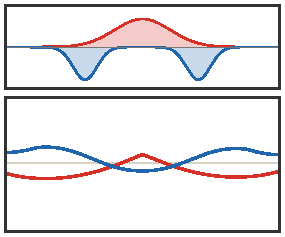
\includegraphics[width=.30\linewidth]{figures/dual-kantorovich-continuous-potentials/target-balanced.pdf} &

\includegraphics[width=.30\linewidth]{figures/dual-kantorovich-continuous-potentials/target-shifted.pdf} &
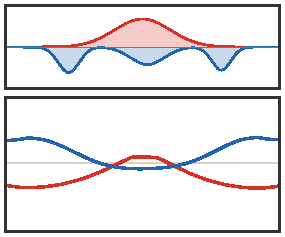
\includegraphics[width=.30\linewidth]{figures/dual-kantorovich-continuous-potentials/target-three-mode.pdf} \\[-.1em]
\small balanced target &
\small strongly shifted target &
\small three-mode target
\end{tabular}
\caption{Continuous Kantorovich potentials for the same source and target families as Figure~\ref{fig:dual-kantorovich-discrete-potentials}.  The upper strips show the source density $\al$ in red and the target density $\be$ in blue, including the strongly shifted and three-mode targets.  The lower strips show potentials $f$ and $g=f^c$ for the quadratic cost $c(x,y)=|x-y|^2$, with the same gauge convention as in the discrete figure.  The equality set $f(x)+g(y)=c(x,y)$ contains the monotone transport graph.}
\index{Kantorovich!potential}% strictindex
\index{cost!quadratic}% strictindex
\label{fig:dual-kantorovich-continuous-potentials}
\end{figure}

Note that in contrast to the primal problem~\eqref{eq-mk-generic}, showing the existence of solutions to~\eqref{eq-dual-generic} is non-trivial, because the constraint set $\Potentials(\c)$ is not compact and the objective is not coercive. Using the machinery of $c$-transforms detailed in Section~\ref{sec-c-transfo}, one can show that optimal $(\f,\g)$ are necessarily Lipschitz regular, which enables the replacement of the constraint by a compact one.
\index{c-transform}% strictindex


%%%%%%%%%%%%%%%%%%%%%%%%%%%%%%%%%%%%%%%%%%%%%%%%%%%%%%%%%%%%%%%%%%%%%%%%%%%
\section[c-transforms]{$c$-transforms}
\index{c-transform}% strictindex
\label{sec-c-transfo}

The $c$-transform is the operation that improves potentials without changing feasibility. It is both a proof device for dual attainment and the route from duality to Brenier's convex potentials.
\index{dual!attainment}% strictindex
\index{convex!potential}% strictindex

%%%%
\paragraph{Best-response potentials and the $c$-transform.}
\index{c-transform}% strictindex

Keeping a dual potential $\f$ fixed, one can maximize in closed form over the second potential in the dual problem~\eqref{eq-dual-generic}, which leads one to consider
\index{dual!potential}% strictindex
\index{dual!problem}% strictindex
\eq{
	\usup{\g \in \Cc(\Yy)} \enscond{
		\int g \d \be }{
			\foralls (x,y), \g(y) \leq c(x,y) - \f(x)
		}.
}
The constraint can be replaced by
\eq{
	\foralls y \in \Yy, \quad \g(y) \leq \f^\c(y)
}.

\begin{defn}[$c$-transform]\label{def-c-transform}
\index{c-transform}% strictindex
	For a function $f:\Xx\to\RR\cup\{-\infty\}$, its $c$-transform is
	\eql{\label{eq-c-transform}
		\foralls y \in \Y, \quad
		\f^\c(y) \eqdef \uinf{x \in \X} \c(x,y) - \f(x).
	}
	For a function $g:\Yy\to\RR\cup\{-\infty\}$, the $\bar c$-transform associated with $\bar c(y,x)=c(x,y)$ is
	\[
		\foralls x \in \X, \quad
		\g^{\bar\c}(x) \eqdef \uinf{y \in \Y} \c(x,y) - \g(y).
	\]
\end{defn}
Since $\be$ is positive, the maximization of $\int \g \d \be$ is thus achieved at those functions such that $\g=\f^\c$ on the support of $\be$, which means $\be$-almost everywhere.

\begin{figure}[H]
\centering
\begin{tabular}{@{}ccc@{}}
\small $p=1$ &
\small $p=2$ &
\small $p=4$ \\[-.15em]

\includegraphics[width=.30\linewidth]{figures/dual-c-transform-envelope/p1.pdf} &
\index{c-transform}% strictindex
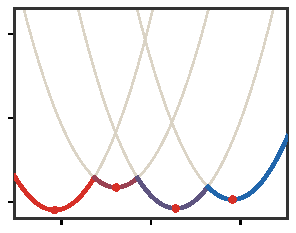
\includegraphics[width=.30\linewidth]{figures/dual-c-transform-envelope/p2.pdf} &

\includegraphics[width=.30\linewidth]{figures/dual-c-transform-envelope/p4.pdf}
\end{tabular}
\caption{Discrete $c$-transform as a lower envelope for costs $c_p(x,y)=|x-y|^p$.  The red circles are four source atoms $x_i$ with potential values $f_i$; the gray curves are the translated functions $y\mapsto c_p(x_i,y)-f_i$; the colored curve is their lower envelope $f^c(y)=\min_i c_p(x_i,y)-f_i$. This is the semi-discrete situation where $\X$ is finite, equivalently the source measure $\al$ is discrete; Chapter~\ref{sec-semidiscr-w1} studies the complementary case where the eliminated potential is supported on finitely many target atoms.}
\index{semi-discrete!OT}% strictindex
\index{c-transform}% strictindex
\label{fig:dual-c-transform-envelope}
\end{figure}

\begin{prop}[$c$-transforms solve the semi-relaxed problems]\label{prop-c-transform-semi-relaxed}
\index{c-transform}% strictindex
\index{semi-relaxed!problem}% strictindex
	For fixed $f$, the maximizers of the dual objective over all $g$ such that $f\oplus g\leq c$ are exactly the functions satisfying $g=f^c$ $\be$-almost everywhere. Equivalently, $f^c$ gives the value of the one-marginal primal problem
	\[
		\inf_{\pi:\,\pi_2=\be}
		\int c(x,y)\d\pi(x,y)-\int f(x)\d\pi_1(x)
		=
		\int f^c(y)\d\be(y).
	\]
	Symmetrically, for fixed $g$, the maximizers over $f$ are the functions satisfying $f=g^{\bar c}$ $\al$-almost everywhere.
\end{prop}
\begin{proof}
	The constraint $f(x)+g(y)\leq c(x,y)$ for all $x$ is equivalent, for each fixed $y$, to
	\[
		g(y)\leq \inf_x c(x,y)-f(x)=f^c(y).
	\]
	Since $\be$ is nonnegative, the largest possible value of $\int g\d\be$ is obtained by saturating this pointwise upper bound on the support of $\be$. The proof for $f=g^{\bar c}$ is identical after exchanging the two marginals.

	For the primal formula, disintegrate any feasible $\pi$ as $\pi(\d x,\d y)=\pi_y(\d x)\be(\d y)$. Then
\index{disintegration}% strictindex
	\[
		\int c\d\pi-\int f\d\pi_1
		=
		\int\left(\int (c(x,y)-f(x))\d\pi_y(x)\right)\d\be(y)
		\geq
		\int f^c(y)\d\be(y).
	\]
	If minimizers admit a measurable selection, equality is obtained by choosing $\pi_y$ supported on minimizers of $x\mapsto c(x,y)-f(x)$. Otherwise one uses approximate measurable selections and lets the approximation error vanish.
\index{measurable selection}% strictindex
\end{proof}

The map $(f,g)\mapsto(g^{\bar c},f^c)$ replaces dual potentials by better ones, in the sense that it preserves feasibility and improves the dual objective. Functions of the form $f^c$ and $g^{\bar c}$ are called $c$-concave and $\bar c$-concave functions. These partial minimizations define maximizers on the supports of $\al$ and $\be$, while Definition~\ref{def-c-transform} defines functions on the whole spaces $\X$ and $\Y$. This gives a canonical extension of dual solutions beyond the active supports.
\index{dual!potential}% strictindex
\index{c-transform}% strictindex

\begin{prop}[Lipschitz stability of $c$-transforms]\label{prop-c-transform-lipschitz}
\index{Lipschitz stability}% strictindex
\index{Lipschitz!stability}% strictindex
\index{c-transform}% strictindex
	If $c$ is $L$-Lipschitz with respect to its second variable, uniformly in the first one and for the metric $d_\Y$ on $\Y$, then $f^c$ is $L$-Lipschitz.
\end{prop}
\begin{proof}
	For each $x$, set $F_x(y)=c(x,y)-f(x)$ and $F(y)=f^c(y)=\inf_x F_x(y)$. Since all the functions $F_x$ are $L$-Lipschitz,
	\[
		|F(y)-F(y')|
		=
		\left|\inf_x F_x(y)-\inf_x F_x(y')\right|
		\leq
		\sup_x |F_x(y)-F_x(y')|
		\leq
		L d_\Y(y,y').
	\]
\end{proof}

This stability is crucial for dual attainment. When $c$ is Lipschitz on compact spaces, one can replace arbitrary admissible potentials by $c$-transformed ones with a uniform Lipschitz bound; after fixing the harmless additive gauge, compactness follows from the Arzela--Ascoli theorem.
\index{dual!attainment}% strictindex

\paragraph{Euclidean case.}

The Euclidean quadratic cost is the model case where $c$-transforms become ordinary convex conjugates after removing the quadratic terms. This is the algebraic bridge between Kantorovich duality and Brenier maps.
\index{Kantorovich!duality}% strictindex
\index{convex!conjugate}% strictindex
\index{cost!quadratic}% strictindex
\index{Brenier!map}% strictindex
\index{c-transform}% strictindex

The special cost $c(x,y)=-\dotp{x}{y}$ on $\X=\Y=\RR^d$ is central because it reduces the quadratic Wasserstein problem to convex duality. Indeed, for any $\pi\in\Couplings(\al,\be)$,
\[
	\int \norm{x-y}^2\d\pi(x,y)
	=
	\int\norm{x}^2\d\al(x)+\int\norm{y}^2\d\be(y)
	-2\int \dotp{x}{y}\d\pi(x,y).
\]
For $c(x,y)=-\dotp{x}{y}$, one has
\[
	f^c(y)
	=
	\inf_x -\dotp{x}{y}-f(x)
	=
	-(-f)^*(y),
	\qquad
	h^*(y)\eqdef\sup_x \dotp{x}{y}-h(x).
\]
Thus $c$-concave functions are negatives of convex functions. In the one-dimensional bilinear model case, the hard double $c$-transform is therefore an operation of taking concave envelopes.
\index{convex!function}% strictindex
\index{c-transform}% strictindex

\begin{rem}[Proof of Brenier's theorem]\label{rem-proof-brenier}
\index{Brenier!theorem}% strictindex
	For $c(x,y)=\norm{x-y}^2$, subtracting the harmless quadratic terms reduces the geometry to the bilinear cost $-\dotp{x}{y}$. The primal-dual relationship, together with the fact that one can replace $(f,g)$ by $(f^{c\bar c},f^c)$, shows that an optimal plan satisfies
\index{optimal plan}% strictindex
	\[
		\supp(\pi)
		\subset
		\enscond{(x,y)}{\phi(x)+\phi^*(y)=\dotp{x}{y}},
	\]
	where $\phi=-f^{c\bar c}$ is convex and $-g=\phi^*$. By the Fenchel inequality, equality holds exactly when $y\in\partial\phi(x)$. If $\al$ has a density, convex functions are differentiable Lebesgue-almost everywhere, hence $\al$-almost everywhere, so $\partial\phi(x)$ is a singleton for $\al$-almost every $x$. This yields the Brenier map $T=\nabla\phi$ and explains why the optimal coupling is concentrated on a graph.
\index{optimal coupling}% strictindex
\index{convex!function}% strictindex
\index{Brenier!map}% strictindex
\end{rem}


%%%%
\paragraph{The failure of alternate optimization.}
\index{alternate optimization}% strictindex
\index{alternating optimization}% strictindex

A crucial property of the Legendre transform is that $f^{***}=f^*$, and that $f^{**}$ is the convex envelope of $f$ (the largest convex function below $f$). These properties carry over for the more general setting of $c$-transforms. The required convex-analytic background is standard in Rockafellar's theory~\cite{rockafellar2015convex}.
\index{convex envelope}% strictindex
\index{convex!function}% strictindex
\index{Legendre transform}% strictindex
\index{c-transform}% strictindex

\begin{prop}[Algebra of $c$-transforms]
\index{c-transform}% strictindex
The following identities, in which the inequality sign between vectors should be understood elementwise, hold, denoting $\f^{c\bar c} \eqdef (\f^{c})^{\bar c}$:
	\[
		\textnormal{(i) } f \leq f' \Rightarrow f^{c}\geq f'^{c},
		\qquad
		\textnormal{(ii) } f^{\c\bar{\c}} \geq f,
		\qquad
		\textnormal{(iii) } g^{\bar{\c}\c} \geq g,
		\qquad
		\textnormal{(iv) } \f^{\c\bar{\c}\c}=\f^{\c}.
	\]
\end{prop}

\begin{proof} The first inequality (i) follows from the definition of $\c$-transforms (because of the $-$ sign). To prove (ii), expanding the definition of $\f^{\c\bar{\c}}$ we have
\eq{
	\left(\f^{\c\bar{\c}}\right)(x)= \min_{y} \c(x,y)-\f^{\c}(y)
		= \min_{y} \c(x,y) - \min_{x'}( \c(x',y) - \f(x') ).}
Now, since $-\min_{x'}\big(\c(x',y)-\f(x')\big) \geq -(\c(x,y)-\f(x))$, we recover
\eq{
	(\f^{\c\bar{\c}})(x) \geq \min_{y} \c(x,y) - \c(x,y)+\f(x) = \f(x).
}
The relation $\g^{\bar{\c}\c} \geq \g$ is obtained in the same way.
%
Now, to prove (iv), we first apply (ii) and then (i) with $f'=f^{c\bar c}$ to have $f^c \geq f^{c \bar c c}$.
Then we apply (iii) to $g=f^c$ to obtain $f^c \leq f^{c\bar c c}$.
%we apply (ii) to $\g=\f^{\c}$ to obtain
% set $\g=\f^{\c}$. Then, using (ii), $\g^{\bar{\c}}=\f^{\c\bar{\c}}\geq \f$. Therefore, using result (i) we have $\f^{\c\bar{\c}\c}\leq \f^{\c}$. Result (ii) yields $\f^{\c\bar{\c}\c}\geq \f^{\c}$, proving the equality.
\end{proof}

This invariance property shows that one can ``improve'' only once the dual potential this way. Indeed, starting from any pair $(f,g)$, one obtains the following iterates by alternating maximization
\index{dual!potential}% strictindex
\eql{\label{eq-iter-c-trans}
	(f,g) \mapsto (f,f^c) \mapsto (f^{c\bar c},f^c) \mapsto (f^{c\bar c},f^{c\bar c c}) =  (f^{c\bar c},f^c) \ldots
}
so that one reaches a stationary point.
\index{stationarity}% strictindex

\begin{alg}[Hard alternating $c$-transform closure]\label{alg:hard-c-transform-closure}
\index{c-transform}% strictindex
\textbf{Input:} Source potential $f$ on $\X$, cost $c$.

\textbf{Output:} Closed $c$-concave pair $(\tilde f,\tilde g)$.

\textbf{Set} target best response:
\[
	g=f^c,
	\qquad
	g(y)=\inf_{x\in\X}\ c(x,y)-f(x).
\]
\textbf{Set} source closure:
\[
	\tilde f=g^{\bar c}=f^{c\bar c}.
\]
\textbf{Set} closed target potential:
\[
	\tilde g=\tilde f^c=f^{c\bar c c}=f^c.
\]
\textbf{Return} $(\tilde f,\tilde g)=(f^{c\bar c},f^c)$.
\end{alg}

%
This failure is the classical behavior of alternating maximization on a non-smooth problem, where the non-smooth part of the functional (here the constraint) mixes the two variables.
%
The workaround is to introduce smoothing, which is the classical method of augmented Lagrangian, and that we will develop here using entropic regularization, which corresponds to Sinkhorn's algorithm.
\index{Sinkhorn!algorithm}% strictindex
\index{entropic!regularization}% strictindex

For the bilinear cost $c(x,y)=-xy$ on a compact interval, the $c$-concave functions are ordinary concave functions and $f^{c\bar c}$ is the smallest concave majorant of $f$. In that model case, a hard transform removes non-concave oscillations in one closure step rather than producing a gradual ascent.

\begin{figure}[ht]
\centering
\begin{tabular}{@{}cc@{}}

\includegraphics[width=.46\linewidth]{figures/dual-alternating-c-transform-failure/source-concave-closure.pdf} &
\index{c-transform}% strictindex

\includegraphics[width=.46\linewidth]{figures/dual-alternating-c-transform-failure/target-concave-closure.pdf} \\[-.1em]
\small source-side closure & \small target-side closure
\end{tabular}
\caption{Hard $c$-transforms for the bilinear cost $c(x,y)=-xy$. The source-side panel uses a reddish palette and starts from a sharply oscillatory potential $f$; the target-side panel uses a blueish palette and starts from a visually different potential $g$. Dark curves are the double-transform closures $f^{c\bar c}$ and $g^{\bar c c}$, which are concave majorants, while dashed lighter curves are the one-sided best responses $g^{\bar c}$ and $f^c$ after a harmless vertical gauge shift. The figure illustrates why exact alternating best responses are useful for dual certificates but do not give the smooth iterative dynamics later provided by entropic regularization.}
\index{c-transform}% strictindex
\index{entropic!regularization}% strictindex
\index{dual!certificate}% strictindex
\label{fig:dual-alternating-c-transform-failure}
\end{figure}
